\documentclass{standalone}
\usepackage{tikz}
\usetikzlibrary{patterns, positioning}
\usetikzlibrary{shapes.misc}
\usepackage[outline]{contour}
\contourlength{1.5pt} 
\usepackage[sfdefault]{ClearSans} %% option 'sfdefault' activates Clear Sans as the default text font
\usepackage[T1]{fontenc}

\begin{document}
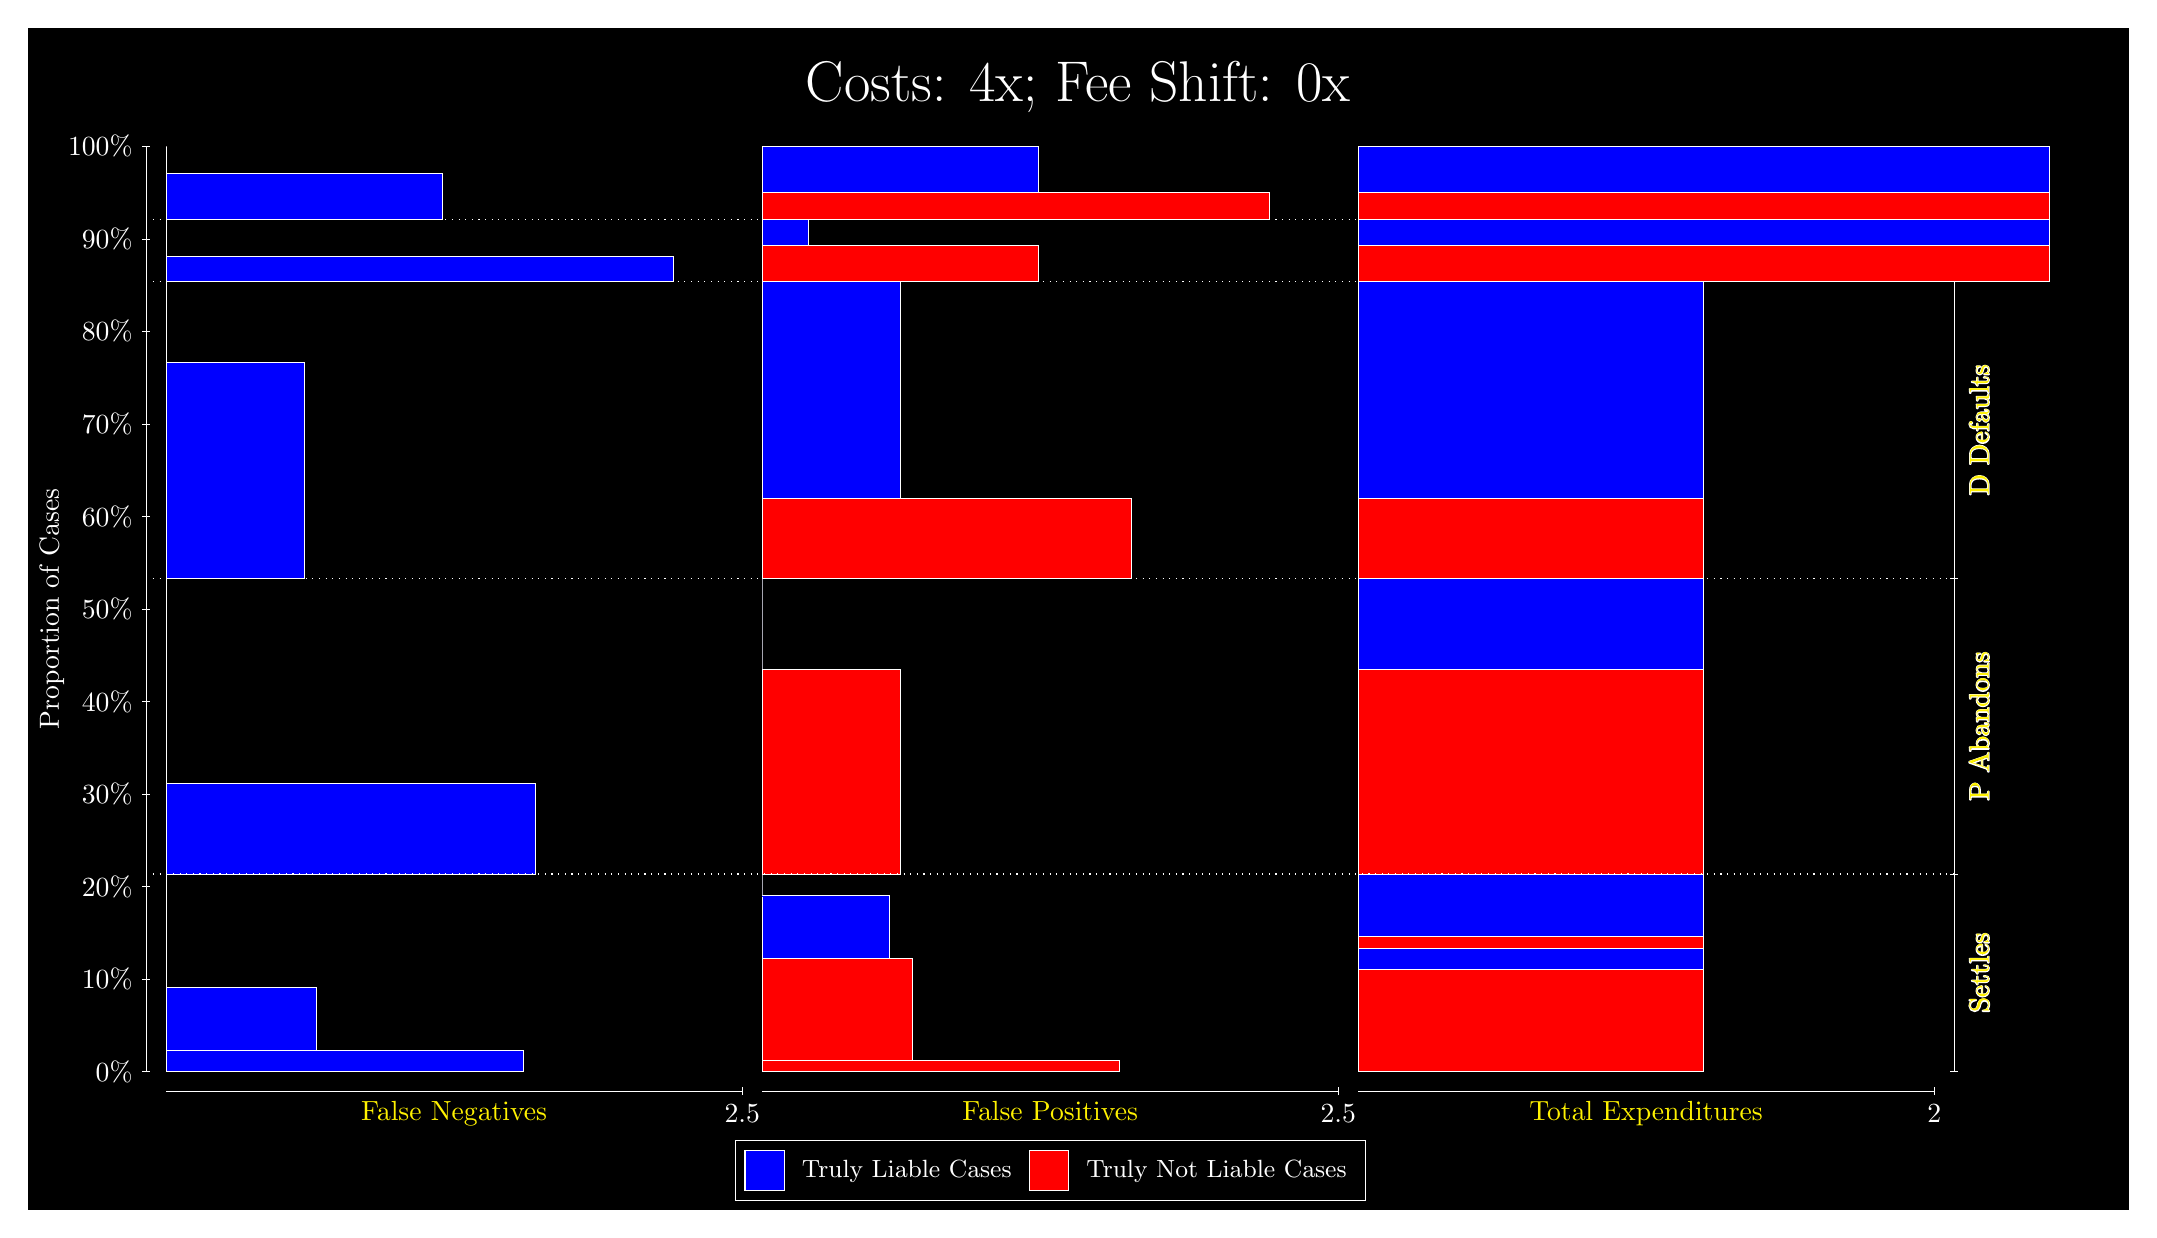
\begin{tikzpicture}
\draw[fill=black] (0,0) rectangle (26.667,15);
\draw[text=white] (0,13.5) rectangle (26.667,15) node[midway] {\huge Costs: 4x; Fee Shift: 0x};
\draw[white, very thin] (1.5,1.75) -- (1.5,13.5);
\node[rotate=90, text=white, anchor=center] at (0.3, 7.625) {Proportion of Cases};
\draw[white, very thin] (1.45,1.75) -- (1.55,1.75);
\node[text=white, anchor=east] at (1.45, 1.75) {0\%};
\draw[white, very thin] (1.45,2.925) -- (1.55,2.925);
\node[text=white, anchor=east] at (1.45, 2.925) {10\%};
\draw[white, very thin] (1.45,4.1) -- (1.55,4.1);
\node[text=white, anchor=east] at (1.45, 4.1) {20\%};
\draw[white, very thin] (1.45,5.275) -- (1.55,5.275);
\node[text=white, anchor=east] at (1.45, 5.275) {30\%};
\draw[white, very thin] (1.45,6.45) -- (1.55,6.45);
\node[text=white, anchor=east] at (1.45, 6.45) {40\%};
\draw[white, very thin] (1.45,7.625) -- (1.55,7.625);
\node[text=white, anchor=east] at (1.45, 7.625) {50\%};
\draw[white, very thin] (1.45,8.8) -- (1.55,8.8);
\node[text=white, anchor=east] at (1.45, 8.8) {60\%};
\draw[white, very thin] (1.45,9.975) -- (1.55,9.975);
\node[text=white, anchor=east] at (1.45, 9.975) {70\%};
\draw[white, very thin] (1.45,11.15) -- (1.55,11.15);
\node[text=white, anchor=east] at (1.45, 11.15) {80\%};
\draw[white, very thin] (1.45,12.325) -- (1.55,12.325);
\node[text=white, anchor=east] at (1.45, 12.325) {90\%};
\draw[white, very thin] (1.45,13.5) -- (1.55,13.5);
\node[text=white, anchor=east] at (1.45, 13.5) {100\%};

\draw[white, very thin] (24.457,1.75) -- (24.457,13.5);
\draw[white, very thin] (24.407,1.75) -- (24.507,1.75);
\node[anchor=west] at (24.407, 1.75) {};
\draw[white, very thin] (24.407,4.258) -- (24.507,4.258);
\node[anchor=west] at (24.407, 4.258) {};
\draw[white, very thin] (24.407,8.0128) -- (24.507,8.0128);
\node[anchor=west] at (24.407, 8.0128) {};
\draw[white, very thin] (24.407,11.782) -- (24.507,11.782);
\node[anchor=west] at (24.407, 11.782) {};
\draw[white, very thin] (24.407,12.572) -- (24.507,12.572);
\node[anchor=west] at (24.407, 12.572) {};
\draw[white, very thin] (24.407,13.5) -- (24.507,13.5);
\node[anchor=west] at (24.407, 13.5) {};

\draw[white, very thin, fill=blue] (1.75,1.75) rectangle (6.2877,2.0234);
\draw[white, very thin, fill=blue] (1.75,2.0234) rectangle (4.9703,2.0252);
\draw[white, very thin, fill=blue] (1.75,2.0252) rectangle (3.6529,2.82);
\draw[white, very thin, fill=red] (1.75,2.82) rectangle (1.75,4.258);
\draw[white, very thin, fill=blue] (1.75,4.258) rectangle (6.4341,5.4064);
\draw[white, very thin, fill=red] (1.75,5.4064) rectangle (1.75,8.0128);
\draw[white, very thin, fill=blue] (1.75,8.0128) rectangle (3.5065,10.761);
\draw[white, very thin, fill=red] (1.75,10.761) rectangle (1.75,11.782);
\draw[white, very thin, fill=blue] (1.75,11.782) rectangle (8.1906,12.109);
\draw[white, very thin, fill=red] (1.75,12.109) rectangle (1.75,12.572);
\draw[white, very thin, fill=blue] (1.75,12.572) rectangle (5.2631,13.154);
\draw[white, very thin, fill=red] (1.75,13.154) rectangle (1.75,13.5);
\draw[white, very thin, fill=red] (9.3189,1.75) rectangle (13.857,1.8972);
\draw[white, very thin, fill=red] (9.3189,1.8972) rectangle (12.539,1.8987);
\draw[white, very thin, fill=red] (9.3189,1.8987) rectangle (11.222,3.188);
\draw[white, very thin, fill=blue] (9.3189,3.188) rectangle (10.929,3.9828);
\draw[white, very thin, fill=blue] (9.3189,3.9828) rectangle (9.6116,3.9846);
\draw[white, very thin, fill=blue] (9.3189,3.9846) rectangle (9.3189,4.258);
\draw[white, very thin, fill=red] (9.3189,4.258) rectangle (11.075,6.8644);
\draw[white, very thin, fill=blue] (9.3189,6.8644) rectangle (9.3189,8.0128);
\draw[white, very thin, fill=red] (9.3189,8.0128) rectangle (14.003,9.0339);
\draw[white, very thin, fill=blue] (9.3189,9.0339) rectangle (11.075,11.782);
\draw[white, very thin, fill=red] (9.3189,11.782) rectangle (12.832,12.246);
\draw[white, very thin, fill=blue] (9.3189,12.246) rectangle (9.9044,12.572);
\draw[white, very thin, fill=red] (9.3189,12.572) rectangle (15.759,12.918);
\draw[white, very thin, fill=blue] (9.3189,12.918) rectangle (12.832,13.5);
\draw[white, very thin, fill=red] (16.888,1.75) rectangle (21.279,1.7515);
\draw[white, very thin, fill=blue] (16.888,1.7515) rectangle (21.279,1.7532);
\draw[white, very thin, fill=red] (16.888,1.7532) rectangle (21.279,3.0426);
\draw[white, very thin, fill=blue] (16.888,3.0426) rectangle (21.279,3.316);
\draw[white, very thin, fill=red] (16.888,3.316) rectangle (21.279,3.4632);
\draw[white, very thin, fill=blue] (16.888,3.4632) rectangle (21.279,4.258);
\draw[white, very thin, fill=red] (16.888,4.258) rectangle (21.279,6.8644);
\draw[white, very thin, fill=blue] (16.888,6.8644) rectangle (21.279,8.0128);
\draw[white, very thin, fill=red] (16.888,8.0128) rectangle (21.279,9.0339);
\draw[white, very thin, fill=blue] (16.888,9.0339) rectangle (21.279,11.782);
\draw[white, very thin, fill=red] (16.888,11.782) rectangle (25.67,12.246);
\draw[white, very thin, fill=blue] (16.888,12.246) rectangle (25.67,12.572);
\draw[white, very thin, fill=red] (16.888,12.572) rectangle (25.67,12.918);
\draw[white, very thin, fill=blue] (16.888,12.918) rectangle (25.67,13.5);
\draw[white, dotted] (1.5,4.258) -- (24.457,4.258);
\draw[white, dotted] (1.5,8.0128) -- (24.457,8.0128);
\draw[white, dotted] (1.5,11.782) -- (24.457,11.782);
\draw[white, dotted] (1.5,12.572) -- (24.457,12.572);
\draw[white, very thin] (1.75,1.5) -- (9.0689,1.5);
\node[text=yellow, anchor=north] at (5.4094, 1.5) {False Negatives};
\draw[white, very thin] (9.0689,1.45) -- (9.0689,1.55);
\node[text=white, anchor=north] at (9.0689, 1.45) {2.5};

\draw[white, very thin] (9.3189,1.5) -- (16.638,1.5);
\node[text=yellow, anchor=north] at (12.978, 1.5) {False Positives};
\draw[white, very thin] (16.638,1.45) -- (16.638,1.55);
\node[text=white, anchor=north] at (16.638, 1.45) {2.5};

\draw[white, very thin] (16.888,1.5) -- (24.207,1.5);
\node[text=yellow, anchor=north] at (20.547, 1.5) {Total Expenditures};
\draw[white, very thin] (24.207,1.45) -- (24.207,1.55);
\node[text=white, anchor=north] at (24.207, 1.45) {2};

\node[text=yellow, centered, rotate=90] at (24.777, 3.004) {\contour{white}{Settles}};
\node[text=yellow, centered, rotate=90] at (24.777, 6.1354) {\contour{white}{P Abandons}};
\node[text=yellow, centered, rotate=90] at (24.777, 9.8975) {\contour{white}{D Defaults}};



\draw (12.978300999999998,1.5) node[draw=none] (baseCoordinate) {};
\begin{scope}[align=center]
        \matrix[scale=0.5, draw=white, below=0.5cm of baseCoordinate, nodes={draw}, column sep=0.1cm]{
            \node[rectangle, draw, minimum width=0.5cm, minimum height=0.5cm, fill=blue] {}; &
            \node[draw=none, font=\small, text=white] (B) {Truly Liable Cases}; &
            \node[rectangle, draw, minimum width=0.5cm, minimum height=0.5cm, fill=red] {}; &
            \node[draw=none, font=\small, text=white] (B) {Truly Not Liable Cases}; \\
            };
\end{scope}

\end{tikzpicture}
\end{document}